\documentclass[crop,tikz]{standalone}
\usetikzlibrary{%
    arrows,
    arrows.meta,
    backgrounds,
    calc,
    decorations.pathreplacing,
    fit,
    matrix,
    positioning,
    scopes,
    shadows
}
\usepackage[linguistics]{forest}
\usepackage[charter]{mathdesign}
\tikzset{headarrow/.style = {-{Latex[length=.5em]}}}
\tikzset{move/.style = {dashed,blue,headarrow}}

\newcommand{\mlex}[2]{\ensuremath{\textrm{#1} ::\thinspace \mathrm{#2}}}
\newcommand{\fsel}[1]{\ensuremath{\mathrm{#1^+}}}
\newcommand{\fcat}[1]{\ensuremath{\mathrm{#1^-}}}
\newcommand{\flcr}[1]{\ensuremath{\mathrm{#1^+}}}
\newcommand{\flce}[1]{\ensuremath{\mathrm{#1^-}}}
\newcommand{\fadj}[1]{\ensuremath{\mathrm{#1^\sim}}}
\newcommand{\Merge}{Merge}
\newcommand{\Move}{Move}
\newcommand{\Adjoin}{Adjoin}

\begin{document}
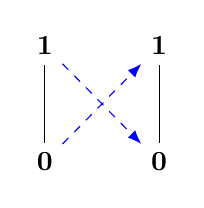
\begin{tikzpicture}
    \node       (l1) at (0,0) {$\mathbf{1}$};
    \node       (l0) [below=of l1] {$\mathbf{0}$};
    \node       (r1) [right=of l1] {$\mathbf{1}$};
    \node       (r0) [below=of r1] {$\mathbf{0}$};

    \foreach \Side in {l, r}
        \draw (\Side 0) to (\Side 1);
    \foreach \Source/\Target in {1/0, 0/1}
        \draw[move] (l\Source) to (r\Target);
\end{tikzpicture}
\end{document}
